% TikZ schematic: U-Net Architecture for Cell Segmentation
% Standalone version - compile with pdflatex
\documentclass[border=10pt]{standalone}
\usepackage{tikz}
\usepackage{xcolor}
\usetikzlibrary{shapes,arrows,positioning,calc,decorations.pathreplacing,patterns,fit,backgrounds}

\definecolor{inputblue}{RGB}{31,119,180}
\definecolor{fftgreen}{RGB}{44,160,44}
\definecolor{featorange}{RGB}{255,127,14}
\definecolor{arrowgray}{RGB}{100,100,100}

\begin{document}
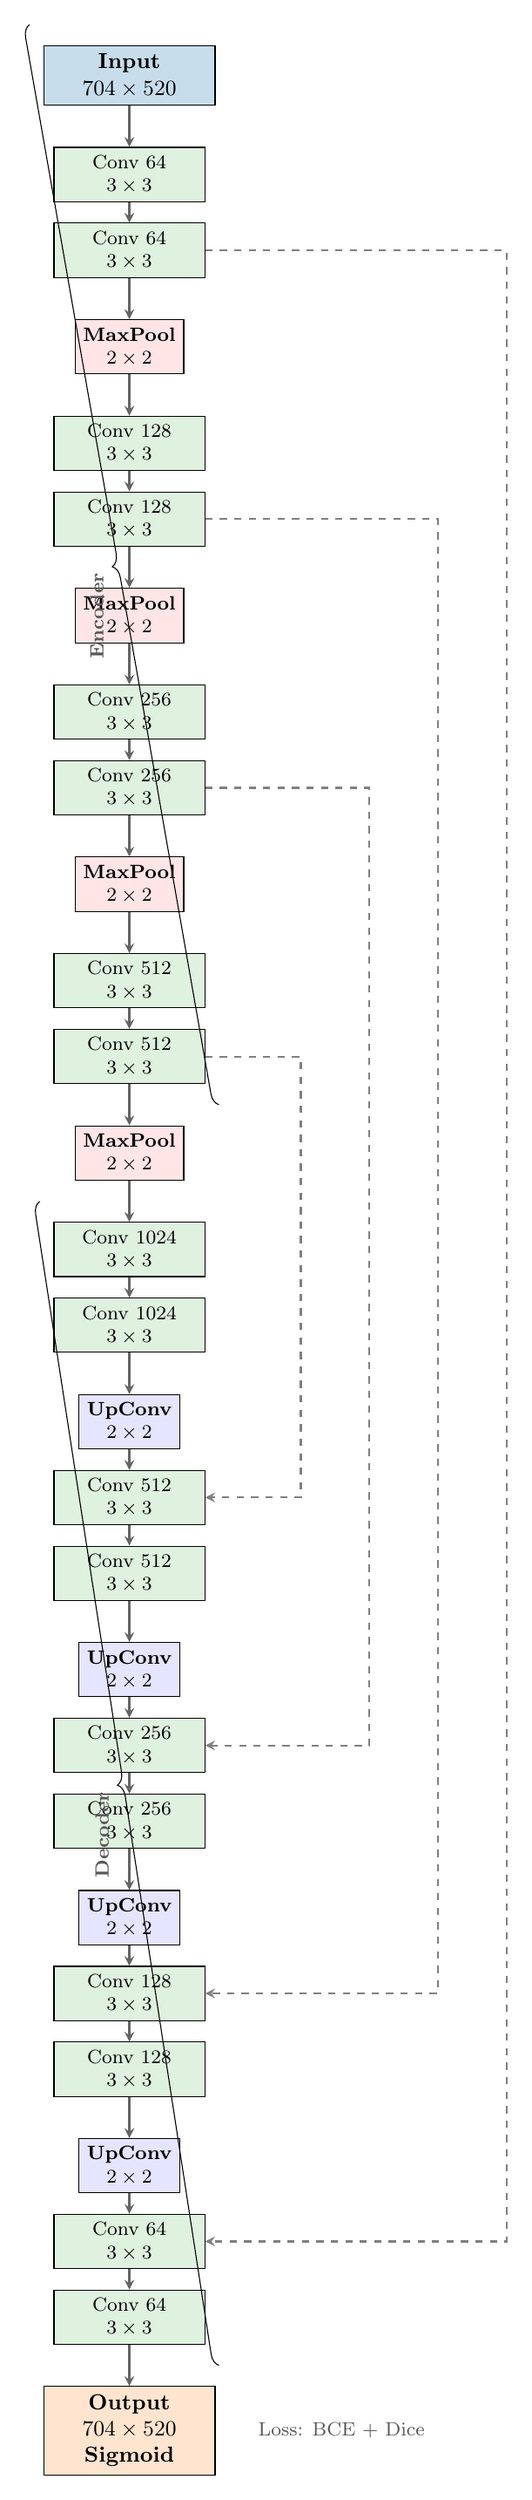
\begin{tikzpicture}[
 node distance=1.2cm and 1.5cm,
 block/.style={rectangle, draw, fill=inputblue!15, minimum width=2.5cm, minimum height=0.8cm, align=center, font=\small\bfseries},
 conv/.style={rectangle, draw, fill=fftgreen!15, minimum width=2.2cm, minimum height=0.7cm, align=center, font=\footnotesize},
 pool/.style={rectangle, draw, fill=red!10, minimum width=1.2cm, minimum height=0.6cm, align=center, font=\footnotesize\bfseries},
 up/.style={rectangle, draw, fill=blue!10, minimum width=1.2cm, minimum height=0.6cm, align=center, font=\footnotesize\bfseries},
 arrow/.style={->, >=stealth, thick, color=arrowgray},
 skip/.style={->, >=stealth, thick, gray, dashed},
 label/.style={font=\footnotesize, color=gray!70!black}
]

% Encoder (left side)
\node[block, fill=inputblue!25] (input) {Input\\$704\times520$}; 
\node[conv, below=0.6cm of input] (conv1) {Conv 64\\$3\times3$}; 
\node[conv, below=0.3cm of conv1] (conv1b) {Conv 64\\$3\times3$}; 
\node[pool, below=0.6cm of conv1b] (pool1) {MaxPool\\$2\times2$}; 

\node[conv, below=0.6cm of pool1] (conv2) {Conv 128\\$3\times3$}; 
\node[conv, below=0.3cm of conv2] (conv2b) {Conv 128\\$3\times3$}; 
\node[pool, below=0.6cm of conv2b] (pool2) {MaxPool\\$2\times2$}; 

\node[conv, below=0.6cm of pool2] (conv3) {Conv 256\\$3\times3$}; 
\node[conv, below=0.3cm of conv3] (conv3b) {Conv 256\\$3\times3$}; 
\node[pool, below=0.6cm of conv3b] (pool3) {MaxPool\\$2\times2$}; 

\node[conv, below=0.6cm of pool3] (conv4) {Conv 512\\$3\times3$}; 
\node[conv, below=0.3cm of conv4] (conv4b) {Conv 512\\$3\times3$}; 
\node[pool, below=0.6cm of conv4b] (pool4) {MaxPool\\$2\times2$}; 

% Bottleneck
\node[conv, below=0.6cm of pool4] (bottle) {Conv 1024\\$3\times3$}; 
\node[conv, below=0.3cm of bottle] (bottleb) {Conv 1024\\$3\times3$}; 

% Decoder (right side)
\node[up, below=0.6cm of bottleb] (up4) {UpConv\\$2\times2$}; 
\node[conv, below=0.3cm of up4] (dconv4) {Conv 512\\$3\times3$}; 
\node[conv, below=0.3cm of dconv4] (dconv4b) {Conv 512\\$3\times3$}; 

\node[up, below=0.6cm of dconv4b] (up3) {UpConv\\$2\times2$}; 
\node[conv, below=0.3cm of up3] (dconv3) {Conv 256\\$3\times3$}; 
\node[conv, below=0.3cm of dconv3] (dconv3b) {Conv 256\\$3\times3$}; 

\node[up, below=0.6cm of dconv3b] (up2) {UpConv\\$2\times2$}; 
\node[conv, below=0.3cm of up2] (dconv2) {Conv 128\\$3\times3$}; 
\node[conv, below=0.3cm of dconv2] (dconv2b) {Conv 128\\$3\times3$}; 

\node[up, below=0.6cm of dconv2b] (up1) {UpConv\\$2\times2$}; 
\node[conv, below=0.3cm of up1] (dconv1) {Conv 64\\$3\times3$}; 
\node[conv, below=0.3cm of dconv1] (dconv1b) {Conv 64\\$3\times3$}; 

% Output
\node[block, fill=featorange!20, below=0.6cm of dconv1b] (output) {Output\\$704\times520$\\Sigmoid}; 

% Arrows - Encoder
\draw[arrow] (input) -- (conv1);
\draw[arrow] (conv1) -- (conv1b);
\draw[arrow] (conv1b) -- (pool1);
\draw[arrow] (pool1) -- (conv2);
\draw[arrow] (conv2) -- (conv2b);
\draw[arrow] (conv2b) -- (pool2);
\draw[arrow] (pool2) -- (conv3);
\draw[arrow] (conv3) -- (conv3b);
\draw[arrow] (conv3b) -- (pool3);
\draw[arrow] (pool3) -- (conv4);
\draw[arrow] (conv4) -- (conv4b);
\draw[arrow] (conv4b) -- (pool4);
\draw[arrow] (pool4) -- (bottle);
\draw[arrow] (bottle) -- (bottleb);

% Arrows - Decoder
\draw[arrow] (bottleb) -- (up4);
\draw[arrow] (up4) -- (dconv4);
\draw[arrow] (dconv4) -- (dconv4b);
\draw[arrow] (dconv4b) -- (up3);
\draw[arrow] (up3) -- (dconv3);
\draw[arrow] (dconv3) -- (dconv3b);
\draw[arrow] (dconv3b) -- (up2);
\draw[arrow] (up2) -- (dconv2);
\draw[arrow] (dconv2) -- (dconv2b);
\draw[arrow] (dconv2b) -- (up1);
\draw[arrow] (up1) -- (dconv1);
\draw[arrow] (dconv1) -- (dconv1b);
\draw[arrow] (dconv1b) -- (output);

% Skip connections
\draw[skip] (conv4b) -- ++(2.5,0) |- (dconv4);
\draw[skip] (conv3b) -- ++(3.5,0) |- (dconv3);
\draw[skip] (conv2b) -- ++(4.5,0) |- (dconv2);
\draw[skip] (conv1b) -- ++(5.5,0) |- (dconv1);

% Brace
\draw[decorate, decoration={brace, amplitude=5pt, mirror}]
 ($(input.north west)+(-0.2,0.3)$) -- ($(conv4b.south east)+(0.2,-0.3)$)
 node[midway, left=0.4cm, label, rotate=90] {\textbf{Encoder}};

\draw[decorate, decoration={brace, amplitude=5pt, mirror}]
 ($(bottle.north west)+(-0.2,0.3)$) -- ($(dconv1b.south east)+(0.2,-0.3)$)
 node[midway, left=0.4cm, label, rotate=90] {\textbf{Decoder}};

% Loss annotation
\node[label, right=0.5cm of output] {Loss: BCE + Dice};

\end{tikzpicture}
\end{document}
